
\section{CF casing heat, gas loss and liner exposure}\label{sec:coupledcf}
The backing now feeds its changing mass, heat storage and through-thickness
conductivity back into the thermal solution. Gas at 2504 K continues to heat
the liner. The resin's two competing rates follow Section~\ref{sec:cfdiag}.
Each casing cell releases gas at its own temperature into an assumed separate
vent. This leaves the liner-side blowing calculation dependent on phenolic
gas alone. The radial model holds the decomposed casing in its original shape.

\begin{table}[H]\centering\begin{tabular}{lrrrrr}\toprule
 & \multicolumn{2}{c}{Half reactive pool [s]} & Casing at & Liner then & Liner gone \\
Motor & Inner cell & Outer cell & 1000 $^\circ$C [s] & [mm] & [s] \\\midrule
Sustainer & 60.7 & 82.4 & 95.1 & 0.45 & 104.3 \\
Booster & 91.4 & 135.3 & 129.7 & 0.40 & 137.9 \\
\bottomrule\end{tabular}\end{table}
\begin{figure}[H]\centering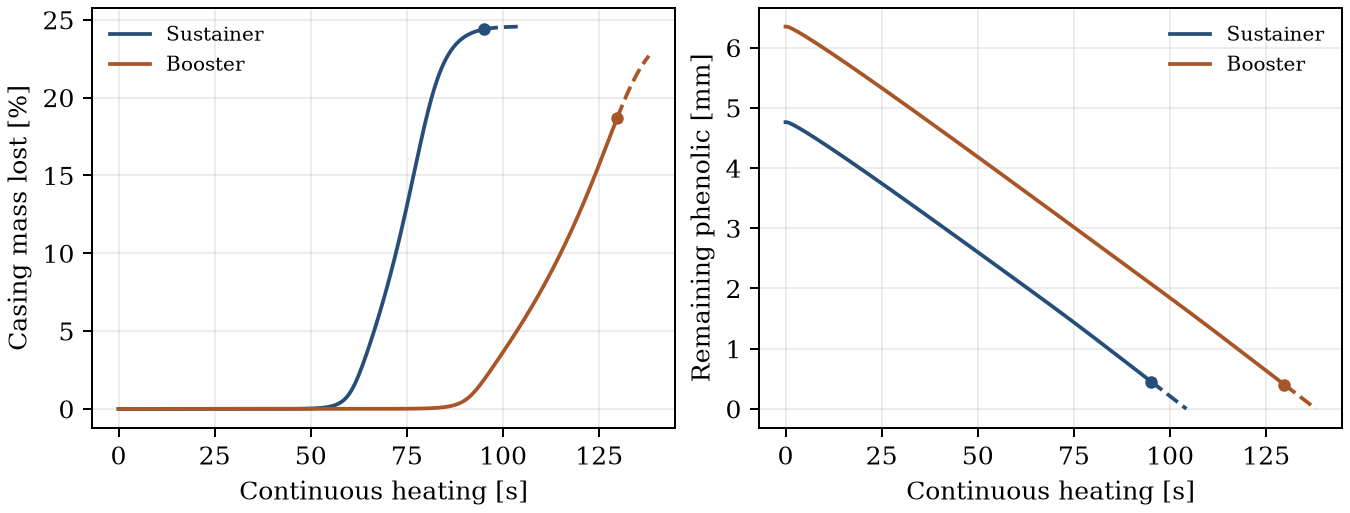
\includegraphics[width=\textwidth]{../analysis/cf_backing_response.png}
\caption{Gas release as a percentage of initial casing mass and remaining liner for the nominal reacting CF
cases. Dots show the first backing temperature of 1000 $^\circ$C. Dashed
segments hold the upper-end residue and gas properties beyond this limit.
Virgin-property fits reach their own limits at lower temperatures.}
\end{figure}
At liner exhaustion the surrogate releases 24.6\% of the sustainer casing
mass and 22.7\% of the booster casing mass. The detailed backing changes the
nominal liner time by +0.32 and +0.28 s respectively relative to the inert
CF baseline. Changing the catalyst coefficient alone shifts these results by
+0.084 and +0.122 s. The local resin, bond and layup in Iris are unknown.
No structural failure time is inferred.

\paragraph{Local thermodynamics.}
For competing extents $a_1,a_2$, define $x=0.554a_1+0.9479a_2$,
$\rho=1575-410x$ in kg/m$^3$ and $\Delta g_i=410\chi_i\Delta a_i V$ in kg.
The remaining cell mass is $m=\rho V$. With sensible enthalpies measured
from 22 $^\circ$C, the reaction substep closes
\[
 (mh_s)_{j+1}-(mh_s)_j=\sum_i Q_i\Delta g_i-h_g(T_{1/2})\sum_i\Delta g_i.
\]
Here $Q_1=+259.54$ and $Q_2=-152.22$ kJ per kg of generated gas, following
the density-loss source in Tranchard et al., Part II. Positive $Q_i$ adds heat.
The model mixes virgin and degraded sensible enthalpies by $x$. Differentiating
this stored energy includes its composition dependence.
\clearpage
\section{CF transport properties and numerical checks}
The model mixes normal conductivity and specific heat between virgin and
degraded states using $x$. For temperature $T$ in $^\circ$C the virgin
fits are $c_v=687.31+2.8773T$ and $k_v=0.61391+0.0011113T$.
The corresponding upper fit limits are 300 and 150 $^\circ$C. The frozen
endpoint value is used outside either fit. The degraded and gas fits below
use a 20--1000 $^\circ$C interval, also with endpoint continuation:
\begin{align*}
 c_d &=662.53+2.599T-2.0761\,10^{-3}T^2+5.1327\,10^{-7}T^3,\\
 k_d &=0.077211+2.3397\,10^{-4}T-4.1903\,10^{-7}T^2+7.4228\,10^{-10}T^3,\\
 c_g &=1256.6+1.0610T-9.2485\,10^{-4}T^2+3.5977\,10^{-7}T^3 .
\end{align*}
Specific heats use J/(kg K) and conductivities W/(m K). Integrating each
bounded heat-capacity function gives its sensible enthalpy. Local radial
conductances include the logarithmic resistance of both adjacent annular
half-cells. The thermal substep iterates conductivity with temperature.
The adiabatic reaction substep advances both pathways against a common
reactant pool and solves for temperature from the open-system energy
equation. A trial repeats at a smaller time step if the reaction fails to
converge or if any cell's total channel advance exceeds 0.04.
The backing vent removes gas enthalpy once at generation. Gas pressure,
internal transport work, swelling and delamination are outside this closure.
\href{https://doi.org/10.3390/ma10050494}{Material measurements, Part I};
\href{https://doi.org/10.3390/ma10050470}{thermal model, Part II}.

\paragraph{Checks.}
A two-cell coupon with a constant outside heat input compares this split solver
against an independent temperature-form ODE. Over 28 s the finest 0.01 s step
gives at most 0.032 K temperature error and 0.0011 absolute error in either
pathway. Both nominal motor pairs pass their mesh and time checks on the
event brackets and remaining thickness. The finest comparisons use 640/160
liner/casing cells and a 0.02 s ceiling. Across the eight runs, each recorded
profile independently reconstructs casing mass and total sensible enthalpy.
An interrupted warm coupon recovered both reaction channels and produced
identical final files after restart. These checks test the specified equations.
Quantitative prediction for Iris still depends on a measured heat load,
recession calibration and material-specific validation.
\clearpage
